\chapter{Algoritmos voraces}

\index{algoritmo voraz}

Un \key{algoritmo voraz}
construye una solución al problema
siempre tomando una elección que parece
ser la mejor en ese momento.
Un algoritmo voraz nunca revierte
sus elecciones, sino que construye directamente
la solución final.
Por esta razón, los algoritmos voraces
suelen ser muy eficientes.

La dificultad en el diseño de algoritmos voraces
es encontrar una estrategia voraz
que siempre produzca una solución óptima
al problema.
Las elecciones localmente óptimas en un algoritmo voraz
también deben ser óptimas a nivel global.
A menudo es difícil argumentar que
un algoritmo voraz funciona.

\section{Problema de monedas}

Como primer ejemplo, consideramos un problema
en el que se nos da un conjunto de monedas
y nuestra tarea es formar una suma de dinero $n$
usando las monedas.
Los valores de las monedas son
$\texttt{monedas}=\{c_1,c_2,\ldots,c_k\}$,
y cada moneda se puede usar tantas veces como queramos.
¿Cuál es el número mínimo de monedas necesario?

Por ejemplo, si las monedas son monedas de euro (en céntimos)
\[\{1,2,5,10,20,50,100,200\}\]
y $n=520$,
necesitamos al menos cuatro monedas.
La solución óptima es seleccionar las monedas
$200+200+100+20$ cuya suma es 520.

\subsubsection{Algoritmo voraz}

Un algoritmo voraz simple para el problema
siempre selecciona la moneda más grande posible,
hasta que se haya construido la suma de dinero requerida.
Este algoritmo funciona en el caso de ejemplo,
porque primero seleccionamos dos monedas de 200 céntimos,
luego una moneda de 100 céntimos y finalmente una moneda de 20 céntimos.
Pero, ¿siempre funciona este algoritmo?

Resulta que si las monedas son monedas de euro,
el algoritmo voraz \emph{siempre} funciona, es decir,
siempre produce una solución con el menor número
posible de monedas.
La corrección del algoritmo se puede
mostrar de la siguiente manera:

Primero, cada moneda 1, 5, 10, 50 y 100 aparece
como máximo una vez en una solución óptima,
porque si la
solución contuviera dos monedas de ese tipo,
podríamos reemplazarlas por una moneda y
obtener una solución mejor.
Por ejemplo, si la solución contuviera
monedas $5+5$, podríamos reemplazarlas por la moneda $10$.

De la misma manera, las monedas 2 y 20 aparecen
como máximo dos veces en una solución óptima,
porque podríamos reemplazar
monedas $2+2+2$ por monedas $5+1$ y
monedas $20+20+20$ por monedas $50+10$.
Además, una solución óptima no puede contener
monedas $2+2+1$ o $20+20+10$,
porque podríamos reemplazarlas por monedas de $5$ y $50$.

Usando estas observaciones,
podemos demostrar para cada moneda $x$ que
no es posible construir de manera óptima
una suma $x$ o cualquier suma mayor utilizando únicamente monedas
que sean más pequeñas que $x$.
Por ejemplo, si $x=100$, la suma óptima más grande
usando monedas más pequeñas es $50+20+20+5+2+2=99$.
Por lo tanto, el algoritmo voraz que siempre selecciona
la moneda más grande produce la solución óptima.

Este ejemplo muestra que puede ser difícil
argumentar que un algoritmo voraz funciona,
incluso si el algoritmo en sí es simple.

\subsubsection{Caso general}

En el caso general, el conjunto de monedas puede contener cualquier moneda
y el algoritmo voraz \emph{no} necesariamente produce
una solución óptima.

Podemos demostrar que un algoritmo voraz no funciona
mostrando un contraejemplo
donde el algoritmo proporciona una respuesta incorrecta.
En este problema, podemos encontrar fácilmente un contraejemplo:
si las monedas son $\{1,3,4\}$ y la suma objetivo
es 6, el algoritmo voraz produce la solución
$4+1+1$ mientras que la solución óptima es $3+3$.

No se sabe si el problema general de las monedas
se puede resolver utilizando algún algoritmo voraz\footnote{Sin embargo, es posible
\emph{verificar} en tiempo polinomial
si el algoritmo voraz presentado en este capítulo funciona para
un conjunto de monedas dado \cite{pea05}.}.
Sin embargo, como veremos en el Capítulo 7,
en algunos casos,
el problema general se puede resolver de manera eficiente
usando un algoritmo de programación dinámica que siempre proporciona la
respuesta correcta.

\section{Planificación}

Muchos problemas de planificación se pueden resolver
utilizando algoritmos voraces.
Un problema clásico es el siguiente:
Dado $n$ eventos con sus horas de inicio y finalización,
encuentra un horario
que incluya la mayor cantidad de eventos posible.
No es posible seleccionar un evento parcialmente.
Por ejemplo, considera los siguientes eventos:
\begin{center}
\begin{tabular}{lll}
evento & hora de inicio & hora de finalización \\
\hline
$A$ & 1 & 3 \\
$B$ & 2 & 5 \\
$C$ & 3 & 9 \\
$D$ & 6 & 8 \\
\end{tabular}
\end{center}
En este caso, el número máximo de eventos es dos.
Por ejemplo, podemos seleccionar los eventos $B$ y $D$
de la siguiente manera:
\begin{center}
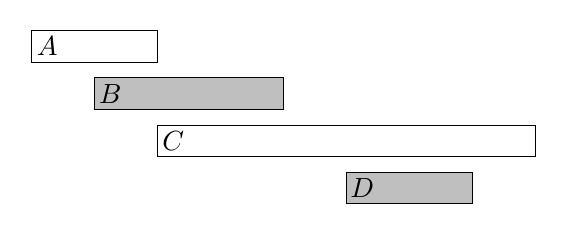
\begin{tikzpicture}[scale=.4]
  \begin{scope}
    \draw (2, 0) rectangle (6, -1);
    \draw[fill=lightgray] (4, -1.5) rectangle (10, -2.5);
    \draw (6, -3) rectangle (18, -4);
    \draw[fill=lightgray] (12, -4.5) rectangle (16, -5.5);
    \node at (2.5,-0.5) {$A$};
    \node at (4.5,-2) {$B$};
    \node at (6.5,-3.5) {$C$};
    \node at (12.5,-5) {$D$};
  \end{scope}
\end{tikzpicture}
\end{center}

Es posible inventar varios algoritmos voraces
para el problema, pero ¿cuál de ellos funciona en todos los casos?

\subsubsection*{Algoritmo 1}

La primera idea es seleccionar eventos lo más \emph{cortos}
posible.
En el caso de ejemplo, este algoritmo
selecciona los siguientes eventos:
\begin{center}
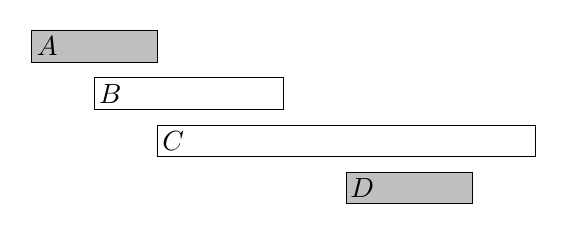
\begin{tikzpicture}[scale=.4]
  \begin{scope}
    \draw[fill=lightgray] (2, 0) rectangle (6, -1);
    \draw (4, -1.5) rectangle (10, -2.5);
    \draw (6, -3) rectangle (18, -4);
    \draw[fill=lightgray] (12, -4.5) rectangle (16, -5.5);
    \node at (2.5,-0.5) {$A$};
    \node at (4.5,-2) {$B$};
    \node at (6.5,-3.5) {$C$};
    \node at (12.5,-5) {$D$};
  \end{scope}
\end{tikzpicture}
\end{center}

Sin embargo, seleccionar eventos cortos no siempre
es una estrategia correcta. Por ejemplo, el algoritmo falla
en el siguiente caso:
\begin{center}
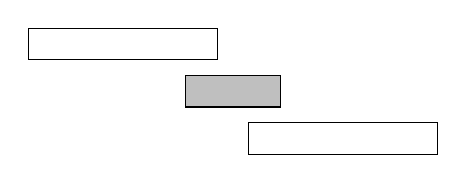
\begin{tikzpicture}[scale=.4]
  \begin{scope}
    \draw (1, 0) rectangle (7, -1);
    \draw[fill=lightgray] (6, -1.5) rectangle (9, -2.5);
    \draw (8, -3) rectangle (14, -4);
  \end{scope}
\end{tikzpicture}
\end{center}
Si seleccionamos el evento corto, solo podemos seleccionar un evento.
Sin embargo, sería posible seleccionar ambos eventos largos.

\subsubsection*{Algoritmo 2}

Otra idea es seleccionar siempre el siguiente evento posible
que \emph{comienza} lo más \emph{temprano} posible.
Este algoritmo selecciona los siguientes eventos:
\begin{center}
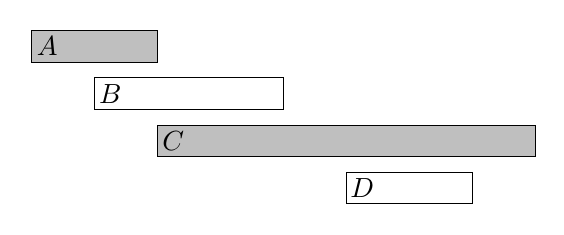
\begin{tikzpicture}[scale=.4]
  \begin{scope}
    \draw[fill=lightgray] (2, 0) rectangle (6, -1);
    \draw (4, -1.5) rectangle (10, -2.5);
    \draw[fill=lightgray] (6, -3) rectangle (18, -4);
    \draw (12, -4.5) rectangle (16, -5.5);
    \node at (2.5,-0.5) {$A$};
    \node at (4.5,-2) {$B$};
    \node at (6.5,-3.5) {$C$};
    \node at (12.5,-5) {$D$};
  \end{scope}
\end{tikzpicture}
\end{center}

Sin embargo, podemos encontrar un contraejemplo
también para este algoritmo.
Por ejemplo, en el siguiente caso,
el algoritmo solo selecciona un evento:
\begin{center}
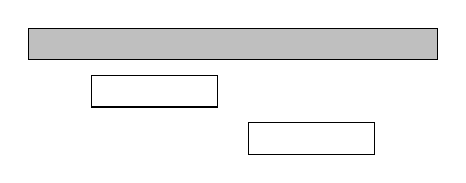
\begin{tikzpicture}[scale=.4]
  \begin{scope}
    \draw[fill=lightgray] (1, 0) rectangle (14, -1);
    \draw (3, -1.5) rectangle (7, -2.5);
    \draw (8, -3) rectangle (12, -4);
  \end{scope}
\end{tikzpicture}
\end{center}
Si seleccionamos el primer evento, no es posible
seleccionar ningún otro evento.
Sin embargo, sería posible seleccionar los
otros dos eventos.

\subsubsection*{Algoritmo 3}

La tercera idea es siempre seleccionar el siguiente
evento posible que \emph{termina} lo más \emph{temprano} posible.
Este algoritmo selecciona los siguientes eventos:
\begin{center}
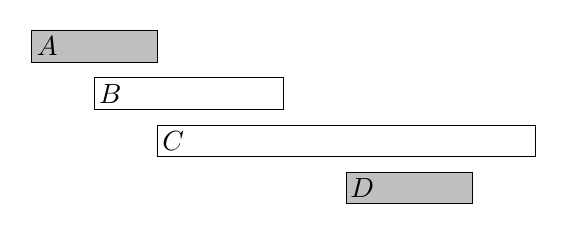
\begin{tikzpicture}[scale=.4]
  \begin{scope}
    \draw[fill=lightgray] (2, 0) rectangle (6, -1);
    \draw (4, -1.5) rectangle (10, -2.5);
    \draw (6, -3) rectangle (18, -4);
    \draw[fill=lightgray] (12, -4.5) rectangle (16, -5.5);
    \node at (2.5,-0.5) {$A$};
    \node at (4.5,-2) {$B$};
    \node at (6.5,-3.5) {$C$};
    \node at (12.5,-5) {$D$};
  \end{scope}
\end{tikzpicture}
\end{center}

Resulta que este algoritmo
\emph{siempre} produce una solución óptima.
La razón de esto es que siempre es una elección óptima
seleccionar primero un evento que termine
lo más temprano posible.
Después de esto, es una elección óptima
seleccionar el siguiente evento
usando la misma estrategia, etc.,
hasta que no podamos seleccionar más eventos.

Una forma de argumentar que el algoritmo funciona
es considerar
qué sucede si primero seleccionamos un evento
que termina más tarde que el evento que termina
lo más temprano posible.
Ahora, tendremos a lo sumo un número igual de
opciones de cómo podemos seleccionar el siguiente evento.
Por lo tanto, seleccionar un evento que termine más tarde
nunca puede generar una solución mejor,
y el algoritmo voraz es correcto.

\section{Tareas y tiempos límite}

Consideremos ahora un problema donde
se nos dan $n$ tareas con duraciones y tiempos límite
y nuestra tarea es elegir un orden para realizar las tareas.
Para cada tarea, ganamos $d-x$ puntos
donde $d$ es el tiempo límite de la tarea
y $x$ es el momento en que terminamos la tarea.
¿Cuál es el mayor puntaje total posible
que podemos obtener?

Por ejemplo, supongamos que las tareas son las siguientes:
\begin{center}
\begin{tabular}{lll}
tarea & duración & tiempo límite \\
\hline
$A$ & 4 & 2 \\
$B$ & 3 & 5 \\
$C$ & 2 & 7 \\
$D$ & 4 & 5 \\
\end{tabular}
\end{center}
En este caso, un programa óptimo para las tareas
es el siguiente:
\begin{center}
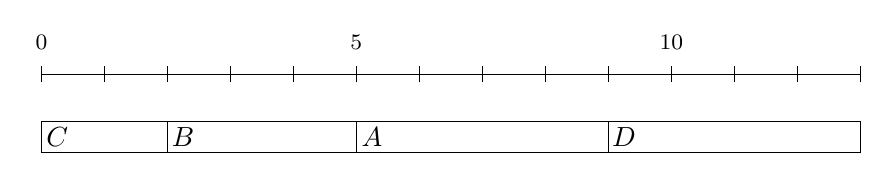
\begin{tikzpicture}[scale=.4]
  \begin{scope}
    \draw (0, 0) rectangle (4, -1);
    \draw (4, 0) rectangle (10, -1);
    \draw (10, 0) rectangle (18, -1);
    \draw (18, 0) rectangle (26, -1);
    \node at (0.5,-0.5) {$C$};
    \node at (4.5,-0.5) {$B$};
    \node at (10.5,-0.5) {$A$};
    \node at (18.5,-0.5) {$D$};

    \draw (0,1.5) -- (26,1.5);
    \foreach \i in {0,2,...,26}
    {
        \draw (\i,1.25) -- (\i,1.75);
    }
    \footnotesize
    \node at (0,2.5) {0};
    \node at (10,2.5) {5};
    \node at (20,2.5) {10};

  \end{scope}
\end{tikzpicture}
\end{center}
En esta solución, $C$ produce 5 puntos,
$B$ produce 0 puntos, $A$ produce $-7$ puntos
y $D$ produce $-8$ puntos,
entonces el puntaje total es $-10$.

Sorprendentemente, la solución óptima al problema
no depende de los tiempos límite en absoluto,
pero una estrategia voraz correcta es simplemente
realizar las tareas \emph{ordenadas por sus duraciones}
en orden creciente.
La razón de esto es que si alguna vez realizamos
dos tareas una tras otra de tal manera que la primera tarea
tarda más que la segunda tarea,
podemos obtener una mejor solución si intercambiamos las tareas.
Por ejemplo, considere el siguiente horario:
\begin{center}
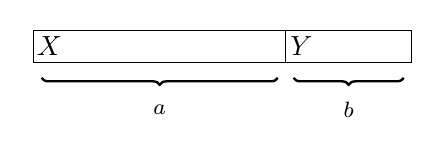
\begin{tikzpicture}[scale=.4]
  \begin{scope}
    \draw (0, 0) rectangle (8, -1);
    \draw (8, 0) rectangle (12, -1);
    \node at (0.5,-0.5) {$X$};
    \node at (8.5,-0.5) {$Y$};

\draw [decoration={brace}, decorate, line width=0.3mm] (7.75,-1.5) -- (0.25,-1.5);
\draw [decoration={brace}, decorate, line width=0.3mm] (11.75,-1.5) -- (8.25,-1.5);

\footnotesize
\node at (4,-2.5) {$a$};
\node at (10,-2.5) {$b$};

  \end{scope}
\end{tikzpicture}
\end{center}
Here $a>b$, so we should swap the tasks:
\begin{center}
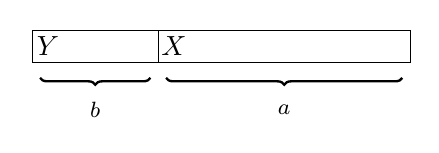
\begin{tikzpicture}[scale=.4]
  \begin{scope}
    \draw (0, 0) rectangle (4, -1);
    \draw (4, 0) rectangle (12, -1);
    \node at (0.5,-0.5) {$Y$};
    \node at (4.5,-0.5) {$X$};

\draw [decoration={brace}, decorate, line width=0.3mm] (3.75,-1.5) -- (0.25,-1.5);
\draw [decoration={brace}, decorate, line width=0.3mm] (11.75,-1.5) -- (4.25,-1.5);

\footnotesize
\node at (2,-2.5) {$b$};
\node at (8,-2.5) {$a$};

  \end{scope}
\end{tikzpicture}
\end{center}
Now $X$ gives $b$ points less and $Y$ gives $a$ points more,
so the total score increases by $a-b > 0$.
In an optimal solution,
for any two consecutive tasks,
it must hold that the shorter task comes
before the longer task.
Thus, the tasks must be performed
sorted by their durations.

\section{Minimizing sums}

We next consider a problem where
we are given $n$ numbers $a_1,a_2,\ldots,a_n$
and our task is to find a value $x$
that minimizes the sum
\[|a_1-x|^c+|a_2-x|^c+\cdots+|a_n-x|^c.\]
We focus on the cases $c=1$ and $c=2$.

\subsubsection{Case $c=1$}

In this case, we should minimize the sum
\[|a_1-x|+|a_2-x|+\cdots+|a_n-x|.\]
For example, if the numbers are $[1,2,9,2,6]$,
the best solution is to select $x=2$
which produces the sum
\[
|1-2|+|2-2|+|9-2|+|2-2|+|6-2|=12.
\]
In the general case, the best choice for $x$
is the \textit{median} of the numbers,
i.e., the middle number after sorting.
For example, the list $[1,2,9,2,6]$
becomes $[1,2,2,6,9]$ after sorting,
so the median is 2.

The median is an optimal choice,
because if $x$ is smaller than the median,
the sum becomes smaller by increasing $x$,
and if $x$ is larger then the median,
the sum becomes smaller by decreasing $x$.
Hence, the optimal solution is that $x$
is the median.
If $n$ is even and there are two medians,
both medians and all values between them
are optimal choices.

\subsubsection{Case $c=2$}

In this case, we should minimize the sum
\[(a_1-x)^2+(a_2-x)^2+\cdots+(a_n-x)^2.\]
For example, if the numbers are $[1,2,9,2,6]$,
the best solution is to select $x=4$
which produces the sum
\[
(1-4)^2+(2-4)^2+(9-4)^2+(2-4)^2+(6-4)^2=46.
\]
In the general case, the best choice for $x$
is the \emph{average} of the numbers.
In the example the average is $(1+2+9+2+6)/5=4$.
This result can be derived by presenting
the sum as follows:
\[
nx^2 - 2x(a_1+a_2+\cdots+a_n) + (a_1^2+a_2^2+\cdots+a_n^2)
\]
The last part does not depend on $x$,
so we can ignore it.
The remaining parts form a function
$nx^2-2xs$ where $s=a_1+a_2+\cdots+a_n$.
This is a parabola opening upwards
with roots $x=0$ and $x=2s/n$,
and the minimum value is the average
of the roots $x=s/n$, i.e.,
the average of the numbers $a_1,a_2,\ldots,a_n$.

\section{Data compression}

\index{data compression}
\index{binary code}
\index{codeword}

A \key{binary code} assigns for each character
of a string a \key{codeword} that consists of bits.
We can \emph{compress} the string using the binary code
by replacing each character by the
corresponding codeword.
For example, the following binary code
assigns codewords for characters
\texttt{A}–\texttt{D}:
\begin{center}
\begin{tabular}{rr}
character & codeword \\
\hline
\texttt{A} & 00 \\
\texttt{B} & 01 \\
\texttt{C} & 10 \\
\texttt{D} & 11 \\
\end{tabular}
\end{center}
This is a \key{constant-length} code
which means that the length of each
codeword is the same.
For example, we can compress the string
\texttt{AABACDACA} as follows:
\[00\,00\,01\,00\,10\,11\,00\,10\,00\]
Using this code, the length of the compressed
string is 18 bits.
However, we can compress the string better
if we use a \key{variable-length} code
where codewords may have different lengths.
Then we can give short codewords for
characters that appear often
and long codewords for characters
that appear rarely.
It turns out that an \key{optimal} code
for the above string is as follows:
\begin{center}
\begin{tabular}{rr}
character & codeword \\
\hline
\texttt{A} & 0 \\
\texttt{B} & 110 \\
\texttt{C} & 10 \\
\texttt{D} & 111 \\
\end{tabular}
\end{center}
An optimal code produces a compressed string
that is as short as possible.
In this case, the compressed string using
the optimal code is
\[0\,0\,110\,0\,10\,111\,0\,10\,0,\]
so only 15 bits are needed instead of 18 bits.
Thus, thanks to a better code it was possible to
save 3 bits in the compressed string.

We require that no codeword
is a prefix of another codeword.
For example, it is not allowed that a code
would contain both codewords 10
and 1011.
The reason for this is that we want
to be able to generate the original string
from the compressed string.
If a codeword could be a prefix of another codeword,
this would not always be possible.
For example, the following code is \emph{not} valid:
\begin{center}
\begin{tabular}{rr}
character & codeword \\
\hline
\texttt{A} & 10 \\
\texttt{B} & 11 \\
\texttt{C} & 1011 \\
\texttt{D} & 111 \\
\end{tabular}
\end{center}
Using this code, it would not be possible to know
if the compressed string 1011 corresponds to
the string \texttt{AB} or the string \texttt{C}.

\index{Huffman coding}

\subsubsection{Huffman coding}

\key{Huffman coding}\footnote{D. A. Huffman discovered this method
when solving a university course assignment
and published the algorithm in 1952 \cite{huf52}.} is a greedy algorithm
that constructs an optimal code for
compressing a given string.
The algorithm builds a binary tree
based on the frequencies of the characters
in the string,
and each character's codeword can be read
by following a path from the root to
the corresponding node.
A move to the left corresponds to bit 0,
and a move to the right corresponds to bit 1.

Initially, each character of the string is
represented by a node whose weight is the
number of times the character occurs in the string.
Then at each step two nodes with minimum weights
are combined by creating
a new node whose weight is the sum of the weights
of the original nodes.
The process continues until all nodes have been combined.

Next we will see how Huffman coding creates
the optimal code for the string
\texttt{AABACDACA}.
Initially, there are four nodes that correspond
to the characters of the string:

\begin{center}
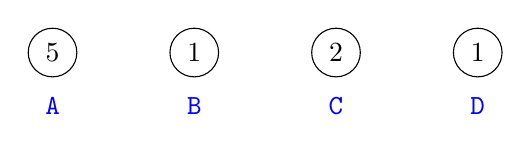
\begin{tikzpicture}[scale=0.9]
\node[draw, circle] (1) at (0,0) {$5$};
\node[draw, circle] (2) at (2,0) {$1$};
\node[draw, circle] (3) at (4,0) {$2$};
\node[draw, circle] (4) at (6,0) {$1$};

\node[color=blue] at (0,-0.75) {\texttt{A}};
\node[color=blue] at (2,-0.75) {\texttt{B}};
\node[color=blue] at (4,-0.75) {\texttt{C}};
\node[color=blue] at (6,-0.75) {\texttt{D}};

%\path[draw,thick,-] (4) -- (5);
\end{tikzpicture}
\end{center}
The node that represents character \texttt{A}
has weight 5 because character \texttt{A}
appears 5 times in the string.
The other weights have been calculated
in the same way.

The first step is to combine the nodes that
correspond to characters \texttt{B} and \texttt{D},
both with weight 1.
The result is:
\begin{center}
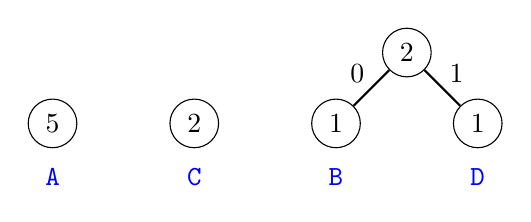
\begin{tikzpicture}[scale=0.9]
\node[draw, circle] (1) at (0,0) {$5$};
\node[draw, circle] (3) at (2,0) {$2$};
\node[draw, circle] (2) at (4,0) {$1$};
\node[draw, circle] (4) at (6,0) {$1$};
\node[draw, circle] (5) at (5,1) {$2$};

\node[color=blue] at (0,-0.75) {\texttt{A}};
\node[color=blue] at (2,-0.75) {\texttt{C}};
\node[color=blue] at (4,-0.75) {\texttt{B}};
\node[color=blue] at (6,-0.75) {\texttt{D}};

\node at (4.3,0.7) {0};
\node at (5.7,0.7) {1};

\path[draw,thick,-] (2) -- (5);
\path[draw,thick,-] (4) -- (5);
\end{tikzpicture}
\end{center}
After this, the nodes with weight 2 are combined:
\begin{center}
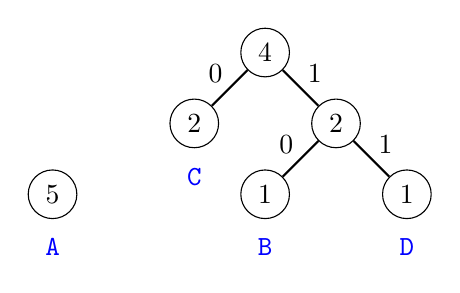
\begin{tikzpicture}[scale=0.9]
\node[draw, circle] (1) at (1,0) {$5$};
\node[draw, circle] (3) at (3,1) {$2$};
\node[draw, circle] (2) at (4,0) {$1$};
\node[draw, circle] (4) at (6,0) {$1$};
\node[draw, circle] (5) at (5,1) {$2$};
\node[draw, circle] (6) at (4,2) {$4$};

\node[color=blue] at (1,-0.75) {\texttt{A}};
\node[color=blue] at (3,1-0.75) {\texttt{C}};
\node[color=blue] at (4,-0.75) {\texttt{B}};
\node[color=blue] at (6,-0.75) {\texttt{D}};

\node at (4.3,0.7) {0};
\node at (5.7,0.7) {1};
\node at (3.3,1.7) {0};
\node at (4.7,1.7) {1};

\path[draw,thick,-] (2) -- (5);
\path[draw,thick,-] (4) -- (5);
\path[draw,thick,-] (3) -- (6);
\path[draw,thick,-] (5) -- (6);
\end{tikzpicture}
\end{center}
Finally, the two remaining nodes are combined:
\begin{center}
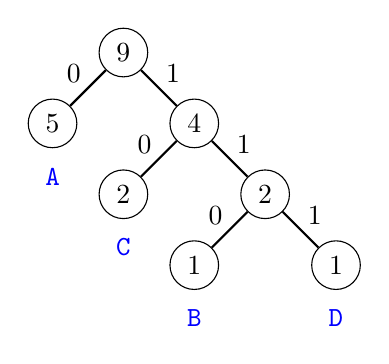
\begin{tikzpicture}[scale=0.9]
\node[draw, circle] (1) at (2,2) {$5$};
\node[draw, circle] (3) at (3,1) {$2$};
\node[draw, circle] (2) at (4,0) {$1$};
\node[draw, circle] (4) at (6,0) {$1$};
\node[draw, circle] (5) at (5,1) {$2$};
\node[draw, circle] (6) at (4,2) {$4$};
\node[draw, circle] (7) at (3,3) {$9$};

\node[color=blue] at (2,2-0.75) {\texttt{A}};
\node[color=blue] at (3,1-0.75) {\texttt{C}};
\node[color=blue] at (4,-0.75) {\texttt{B}};
\node[color=blue] at (6,-0.75) {\texttt{D}};

\node at (4.3,0.7) {0};
\node at (5.7,0.7) {1};
\node at (3.3,1.7) {0};
\node at (4.7,1.7) {1};
\node at (2.3,2.7) {0};
\node at (3.7,2.7) {1};

\path[draw,thick,-] (2) -- (5);
\path[draw,thick,-] (4) -- (5);
\path[draw,thick,-] (3) -- (6);
\path[draw,thick,-] (5) -- (6);
\path[draw,thick,-] (1) -- (7);
\path[draw,thick,-] (6) -- (7);
\end{tikzpicture}
\end{center}

Now all nodes are in the tree, so the code is ready.
The following codewords can be read from the tree:
\begin{center}
\begin{tabular}{rr}
character & codeword \\
\hline
\texttt{A} & 0 \\
\texttt{B} & 110 \\
\texttt{C} & 10 \\
\texttt{D} & 111 \\
\end{tabular}
\end{center}
